%!TEX root = thesis.tex

%:-------------------------- Preamble -----------------------

% Three languages are supported, which will be reflected in the logo on the front page. Pass the appropriate language
% specified as a class option to uit-thesis. Passing any other languages supported by babel will result in the default
% language on the frontpage. If no language is passed, the default is selected.
%  - USenglish (default)
%  - norsk
%  - samin
% The frontpage comes in two variants, Master's thesis and PhD. Master is default, use classoption 'phd' for the PhD version.
\documentclass[USenglish]{uit-thesis}

% Lorem ipsum
\usepackage{lipsum}

\makeglossaries

% Add external glossaryentries
\loadglsentries{acronyms}
\newacronym{api}{API}{application programming interface}\glsunset{api}
\newacronym{2api}{2API}{application programming interface}
\newacronym{d3}{D3}{Data-Driven Documents}
\newacronym{camilla}{CAMILLA}{Camilla is cool!!}
\newacronym{html5}{HTML5}{version 5 of the HyperText Markup Language standard}
\newglossaryentry{thesis}
{
  name=thesis,
  description={is a document submitted in support of candidature for an
    academic degree or professional qualification presenting the author's
    research and findings
    },
}
\newglossaryentry{lage}
{
  name={long ass glossary entry},
  description={is a long ass entry with a lot of text describing the properties of the glossary entry. Hopefully this spans some lines now.
  },
}


\newcommand{\listdefinitionname}{My list of definitions}
\newlistof{definition}{def}{\listdefinitionname}
\newcommand{\definition}[1]{%
  \refstepcounter{definition}%
  \par\noindent\textbf{The Definition~\thedefinition. #1}%
  \addcontentsline{def}{definition}
    {\protect\numberline{\thechapter.\thedefinition}#1}\par%
}

\begin{document}

%:-------------------------- Frontpage ------------------------

\title{From Physical to Virtual Sensors (PVS)}
%\subtitle{Subtitle}			% Optional
\author{Camilla Stormoen}
\thesisfaculty{Faculty of Science and Technology \\ Department of Computer Science}
\thesisprogramme{INF-3983 Capstone Project in Computer Science … December 2017}
%\ThesisFrontpageImage{example_image.jpg}	% Optional

\maketitle

%:-------------------------- Frontmatter -----------------------
\frontmatter

%\begin{dedication}
%To somebody.

%Fuck you very much.
%\end{dedication}

%\begin{epigraph}
%\epigraphitem{Simplicity is prerequisite for reliability.}{Edsger Dijkstra}
%\epigraphitem{Beware of bugs in the above code;\\I have only proved it correct, not tried it.}{Donald Knuth}
%\end{epigraph}

\begin{abstract}
%\lipsum[2-3]
\begin{description}
\item[W3] Whats wrong with the word? / motivation 1-3 setninger
\item[Architecture - 1-3 setninger]
\item [Design- 1-3 setninger]
\item[Implementation - 1-3 setninger]
\item[Experiments - 1-3 setninger]
\item[Results - 1-3 setninger]
\item[Lessons learned/main conclusion - 1-3 setninger]
\item [Kutt heller etterpaa] 
\end{description}

This dissertation present/describe ...
\end{abstract}


%\begin{acknowledgement}
%\lipsum[4-8]
%\end{acknowledgement}

\tableofcontents

\listofdefinition
\listoffigures

%:-------------------------- Mainmatter -----------------------
\mainmatter

\chapter{Introduction}
Introduction to this thesis test! You can start typing!!\cite{coursebook} \\

\section{Motivation}
The motivation!
\begin{itemize}
\item W3
\item Problem definition: This project investegated ... x, with the purpose of y.
\end{itemize}

The motivation  behind this project is that no single sensor may cover the sensing needs, and that sensing needs can change rapidly over time. Consequently, there is a need for sensor fusion, and allow for combining sensors at different computers.

\section{Contributions}
What was the contribution?

\section{Assumptions}
AVGRENSE, VIKTIG!!
Something about motivation and stuff

\section{Limitations}
AVGRENSE, VIKTIG!!

\begin{itemize}
\item The first item .
\item The second item is
\end{itemize}

Some text ...

\begin{enumerate}
\item The first item
\item The second item is a 
\end{enumerate}

\begin{description}
\item[Entry A] with definition A.
\item[Entry B] with definitioin B.
\item[Entry C] with definition C.
\end{description}

\newpage

\subsection{A subsection}

We can use the \ac{api} to \ac{2api} do stuff, and write about what we did in a \gls{thesis}!

This is some stuff, {\sc smallcaps {\em smallcapsemphasized}} {\em regularemphasized}

\Gls{lage}: a test glossary entry.

If the acronym \ac{uit} is displayed, then loadglsentries works.
Hello. This is a test: \ac{camilla}

It is fun to use modern \upsc{OpenMP} technology!\footnote{This is a snarky footnote. Words and etc. Semantic web technologies are technologies that enable semantification of the Web as we know it today. Hopefully this spans some lines now.}

It is fun to use \emph{modern \upsc{OpenMP}} technology! And it is fun to use \ac{d3} and \ac{html5}.

Referencing figure \ref{fig:ex} to test link.\footnote{This is another
footnote.}

\definition{Some other definition}
\definition{Its raining dogs and cats}

%\begin{figure}
%\centering
%
\includegraphics[scale=0.1]{example_image.jpg}
%\caption{Figure link should point to top of figure.}
%\label{fig:ex}
%\end{figure}


\chapter{Background and Related Work}
\begin{itemize}
\item Taking Sensor Networks from the Lab to the Jungle
\item Wireless Sensor Networks for Habitat Monitoring
\item Se de andre paperne Otto har sendt
\end{itemize}

\section{Something}
gggg

\chapter{Architecture}
Functionalities, abstractions, tell it clean/neat.

\begin{figure}
\centering
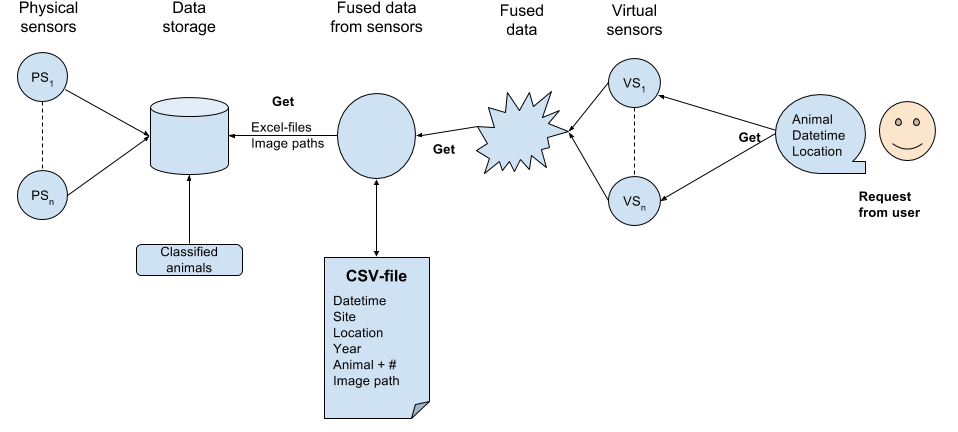
\includegraphics[scale=0.4]{Prosjektoppgave_arkitektur.png}
\caption{Figure showing architecture}
\label{fig:ex}
\end{figure}



We now describe the system architecture, functionality of individual components and how they operate together.
\begin{itemize}
\item Physical sensors??
\item Datastore (DAO)
\item Fused data
\item Virtual sensors
\item Result from virtual sensor to user
\end{itemize}

\chapter{Design}
Client/Server, p2p, put/get, pub/sub, protokoller etc..
BESKRIV INTERAKSJONEN MELLOM ENHETENE!!

Virtual sensors probably uavhengige prosesser, ikke threads ettersom man evt vil addere flere sensorer og unnga a starte alle sensorer på nytt igjen..
Er de virtuelle sensorene servere eller publisher?

\begin{table}
\centering
\begin{tabular}{|l|l|}
\hline
Content left & Content right\\
\hline
\end{tabular}
\caption{A table}
\end{table}

\begin{table}
\centering
\begin{tabular}{|l|l|}
\hline
Content left & Content right\\
\hline
\end{tabular}
\caption{Another table}
\end{table}

\newpage

\begin{lstlisting}[frame=single,caption={Small C program},language=C]
#include "stdio.h"
#define e 3
#define g (e/e)
#define h ((g+e)/2)
#define f (e-g-h)
#define j (e*e-g)
#define k (j-h)
#define l(x) tab2[x]/h
#define m(n,a) ((n&(a))==(a))

long tab1[]={ 989L,5L,26L,0L,88319L,123L,0L,9367L };
int tab2[]={ 4,6,10,14,22,26,34,38,46,58,62,74,82,86 };

main(m1,s) char *s; {
  int a,b,c,d,o[k],n=(int)s;
  if(m1==1){ char b[2*j+f-g]; main(l(h+e)+h+e,b);
    printf(b); }
  else switch(m1-=h){
    case f:
      a=(b=(c=(d=g)<<g)<<g)<<g;
      return(m(n,a|c)|m(n,b)|m(n,a|d)|m(n,c|d));
    case h:
      for(a=f;a<j;++a)
        if(tab1[a]&&!(tab1[a]%((long)l(n))))
          return(a);
    case g:
      if(n<h)return(g);
      if(n<j){n-=g;c='D';o[f]=h;o[g]=f;}
      else{c='\r'-'\b';n-=j-g;o[f]=o[g]=g;}
      if((b=n)>=e)
        for(b=g<<g;b<n;++b)o[b]=o[b-h]+o[b-g]+c;
      return(o[b-g]%n+k-h);
    default:
      if(m1-=e) main(m1-g+e+h,s+g); else *(s+g)=f;
      for(*s=a=f;a<e;) *s=(*s<<e)|main(h+a++,
      (char *)m1);

    }
}
\end{lstlisting}



\chapter{Implementation}
%\lipsum[3-4]
Threads, data structures, language ...
Pandas (dataframe), CV2 (show image), exifread, Python 2.7, missing testing (CPU, memory, time?)

\chapter{Evaluation} 
metrics, define (CPU, memoury, lantecy.), benchmarks (mirko, kernel...
How to measure, where done, PSEUDOCODE
\section{Experimental Setup}
\section{Something!?}
\section{Results}
What does the result say?
Each eksperiemnt, result, meaning

\chapter{Discussion}
Idea, architecture, design, results, andre løsninger, "arch har scaleproblem?"
\section{abcd}

\chapter{Contributions}

\chapter{Conclusion}
\section{Future Work}

\chapter{Future Work?}

\chapter{Appendix?}
readme, source code, dataset measurement RAW
\backmatter


%%% BIBLOGRAPHY

\newpage{}

\begin{thebibliography}{9}

\bibitem{coursebook}
 Robert Sedgewick 
  \emph{Algorithms in C - parts 1-4}.
  Addison-Wesley Publishing Company,
  3. Edition,
  1998.

\end{thebibliography}


\end{document}

